\documentclass[11pt]{article}
\usepackage{sectsty}
\allsectionsfont{\color{blue}\fontfamily{lmss}\selectfont}
\usepackage{fontspec}
\setmainfont{XCharter}

\usepackage{listings}
\lstset{
basicstyle=\small\ttfamily,
tabsize=8,
columns=flexible,
breaklines=true,
frame=tb,
rulecolor=\color[rgb]{0.8,0.8,0.7},
backgroundcolor=\color[rgb]{1,1,0.91},
postbreak=\raisebox{0ex}[0ex][0ex]{\ensuremath{\color{red}\hookrightarrow\space}}
}
\usepackage{fontawesome}


\usepackage{mdframed}
\newmdenv[
  backgroundcolor=gray,
  fontcolor=white,
  nobreak=true,
]{terminalinput}



\usepackage{parskip}


    \usepackage[breakable]{tcolorbox}
    \usepackage{parskip} % Stop auto-indenting (to mimic markdown behaviour)

    \usepackage{iftex}
    \ifPDFTeX
    	\usepackage[T1]{fontenc}
    	\usepackage{mathpazo}
    \else
    	\usepackage{fontspec}
    \fi

    % Basic figure setup, for now with no caption control since it's done
    % automatically by Pandoc (which extracts ![](path) syntax from Markdown).
    \usepackage{graphicx}
    % Maintain compatibility with old templates. Remove in nbconvert 6.0
    \let\Oldincludegraphics\includegraphics
    % Ensure that by default, figures have no caption (until we provide a
    % proper Figure object with a Caption API and a way to capture that
    % in the conversion process - todo).
    \usepackage{caption}
    \DeclareCaptionFormat{nocaption}{}
    \captionsetup{format=nocaption,aboveskip=0pt,belowskip=0pt}

    \usepackage{float}
    \floatplacement{figure}{H} % forces figures to be placed at the correct location
    \usepackage{xcolor} % Allow colors to be defined
    \usepackage{enumerate} % Needed for markdown enumerations to work
    \usepackage{geometry} % Used to adjust the document margins
    \usepackage{amsmath} % Equations
    \usepackage{amssymb} % Equations
    \usepackage{textcomp} % defines textquotesingle
    % Hack from http://tex.stackexchange.com/a/47451/13684:
    \AtBeginDocument{%
        \def\PYZsq{\textquotesingle}% Upright quotes in Pygmentized code
    }
    \usepackage{upquote} % Upright quotes for verbatim code
    \usepackage{eurosym} % defines \euro
    \usepackage[mathletters]{ucs} % Extended unicode (utf-8) support
    \usepackage{fancyvrb} % verbatim replacement that allows latex
    \usepackage{grffile} % extends the file name processing of package graphics
                         % to support a larger range
    \makeatletter % fix for old versions of grffile with XeLaTeX
    \@ifpackagelater{grffile}{2019/11/01}
    {
      % Do nothing on new versions
    }
    {
      \def\Gread@@xetex#1{%
        \IfFileExists{"\Gin@base".bb}%
        {\Gread@eps{\Gin@base.bb}}%
        {\Gread@@xetex@aux#1}%
      }
    }
    \makeatother
    \usepackage[Export]{adjustbox} % Used to constrain images to a maximum size
    \adjustboxset{max size={0.9\linewidth}{0.9\paperheight}}

    % The hyperref package gives us a pdf with properly built
    % internal navigation ('pdf bookmarks' for the table of contents,
    % internal cross-reference links, web links for URLs, etc.)
    \usepackage{hyperref}
    % The default LaTeX title has an obnoxious amount of whitespace. By default,
    % titling removes some of it. It also provides customization options.
    \usepackage{titling}
    \usepackage{longtable} % longtable support required by pandoc >1.10
    \usepackage{booktabs}  % table support for pandoc > 1.12.2
    \usepackage[inline]{enumitem} % IRkernel/repr support (it uses the enumerate* environment)
    \usepackage[normalem]{ulem} % ulem is needed to support strikethroughs (\sout)
                                % normalem makes italics be italics, not underlines
    \usepackage{mathrsfs}



    % Colors for the hyperref package
    \definecolor{urlcolor}{rgb}{0,.145,.698}
    \definecolor{linkcolor}{rgb}{.71,0.21,0.01}
    \definecolor{citecolor}{rgb}{.12,.54,.11}

    % ANSI colors
    \definecolor{ansi-black}{HTML}{3E424D}
    \definecolor{ansi-black-intense}{HTML}{282C36}
    \definecolor{ansi-red}{HTML}{E75C58}
    \definecolor{ansi-red-intense}{HTML}{B22B31}
    \definecolor{ansi-green}{HTML}{00A250}
    \definecolor{ansi-green-intense}{HTML}{007427}
    \definecolor{ansi-yellow}{HTML}{DDB62B}
    \definecolor{ansi-yellow-intense}{HTML}{B27D12}
    \definecolor{ansi-blue}{HTML}{208FFB}
    \definecolor{ansi-blue-intense}{HTML}{0065CA}
    \definecolor{ansi-magenta}{HTML}{D160C4}
    \definecolor{ansi-magenta-intense}{HTML}{A03196}
    \definecolor{ansi-cyan}{HTML}{60C6C8}
    \definecolor{ansi-cyan-intense}{HTML}{258F8F}
    \definecolor{ansi-white}{HTML}{C5C1B4}
    \definecolor{ansi-white-intense}{HTML}{A1A6B2}
    \definecolor{ansi-default-inverse-fg}{HTML}{FFFFFF}
    \definecolor{ansi-default-inverse-bg}{HTML}{000000}

    % common color for the border for error outputs.
    \definecolor{outerrorbackground}{HTML}{FFDFDF}

    % commands and environments needed by pandoc snippets
    % extracted from the output of `pandoc -s`
    \providecommand{\tightlist}{%
      \setlength{\itemsep}{0pt}\setlength{\parskip}{0pt}}
    \DefineVerbatimEnvironment{Highlighting}{Verbatim}{commandchars=\\\{\}}
    % Add ',fontsize=\small' for more characters per line
    \newenvironment{Shaded}{}{}
    \newcommand{\KeywordTok}[1]{\textcolor[rgb]{0.00,0.44,0.13}{\textbf{{#1}}}}
    \newcommand{\DataTypeTok}[1]{\textcolor[rgb]{0.56,0.13,0.00}{{#1}}}
    \newcommand{\DecValTok}[1]{\textcolor[rgb]{0.25,0.63,0.44}{{#1}}}
    \newcommand{\BaseNTok}[1]{\textcolor[rgb]{0.25,0.63,0.44}{{#1}}}
    \newcommand{\FloatTok}[1]{\textcolor[rgb]{0.25,0.63,0.44}{{#1}}}
    \newcommand{\CharTok}[1]{\textcolor[rgb]{0.25,0.44,0.63}{{#1}}}
    \newcommand{\StringTok}[1]{\textcolor[rgb]{0.25,0.44,0.63}{{#1}}}
    \newcommand{\CommentTok}[1]{\textcolor[rgb]{0.38,0.63,0.69}{\textit{{#1}}}}
    \newcommand{\OtherTok}[1]{\textcolor[rgb]{0.00,0.44,0.13}{{#1}}}
    \newcommand{\AlertTok}[1]{\textcolor[rgb]{1.00,0.00,0.00}{\textbf{{#1}}}}
    \newcommand{\FunctionTok}[1]{\textcolor[rgb]{0.02,0.16,0.49}{{#1}}}
    \newcommand{\RegionMarkerTok}[1]{{#1}}
    \newcommand{\ErrorTok}[1]{\textcolor[rgb]{1.00,0.00,0.00}{\textbf{{#1}}}}
    \newcommand{\NormalTok}[1]{{#1}}

    % Additional commands for more recent versions of Pandoc
    \newcommand{\ConstantTok}[1]{\textcolor[rgb]{0.53,0.00,0.00}{{#1}}}
    \newcommand{\SpecialCharTok}[1]{\textcolor[rgb]{0.25,0.44,0.63}{{#1}}}
    \newcommand{\VerbatimStringTok}[1]{\textcolor[rgb]{0.25,0.44,0.63}{{#1}}}
    \newcommand{\SpecialStringTok}[1]{\textcolor[rgb]{0.73,0.40,0.53}{{#1}}}
    \newcommand{\ImportTok}[1]{{#1}}
    \newcommand{\DocumentationTok}[1]{\textcolor[rgb]{0.73,0.13,0.13}{\textit{{#1}}}}
    \newcommand{\AnnotationTok}[1]{\textcolor[rgb]{0.38,0.63,0.69}{\textbf{\textit{{#1}}}}}
    \newcommand{\CommentVarTok}[1]{\textcolor[rgb]{0.38,0.63,0.69}{\textbf{\textit{{#1}}}}}
    \newcommand{\VariableTok}[1]{\textcolor[rgb]{0.10,0.09,0.49}{{#1}}}
    \newcommand{\ControlFlowTok}[1]{\textcolor[rgb]{0.00,0.44,0.13}{\textbf{{#1}}}}
    \newcommand{\OperatorTok}[1]{\textcolor[rgb]{0.40,0.40,0.40}{{#1}}}
    \newcommand{\BuiltInTok}[1]{{#1}}
    \newcommand{\ExtensionTok}[1]{{#1}}
    \newcommand{\PreprocessorTok}[1]{\textcolor[rgb]{0.74,0.48,0.00}{{#1}}}
    \newcommand{\AttributeTok}[1]{\textcolor[rgb]{0.49,0.56,0.16}{{#1}}}
    \newcommand{\InformationTok}[1]{\textcolor[rgb]{0.38,0.63,0.69}{\textbf{\textit{{#1}}}}}
    \newcommand{\WarningTok}[1]{\textcolor[rgb]{0.38,0.63,0.69}{\textbf{\textit{{#1}}}}}


    % Define a nice break command that doesn't care if a line doesn't already
    % exist.
    \def\br{\hspace*{\fill} \\* }
    % Math Jax compatibility definitions
    \def\gt{>}
    \def\lt{<}
    \let\Oldtex\TeX
    \let\Oldlatex\LaTeX
    \renewcommand{\TeX}{\textrm{\Oldtex}}
    \renewcommand{\LaTeX}{\textrm{\Oldlatex}}
    % Document parameters
    % Document title
    \title{index}





% Pygments definitions
\makeatletter
\def\PY@reset{\let\PY@it=\relax \let\PY@bf=\relax%
    \let\PY@ul=\relax \let\PY@tc=\relax%
    \let\PY@bc=\relax \let\PY@ff=\relax}
\def\PY@tok#1{\csname PY@tok@#1\endcsname}
\def\PY@toks#1+{\ifx\relax#1\empty\else%
    \PY@tok{#1}\expandafter\PY@toks\fi}
\def\PY@do#1{\PY@bc{\PY@tc{\PY@ul{%
    \PY@it{\PY@bf{\PY@ff{#1}}}}}}}
\def\PY#1#2{\PY@reset\PY@toks#1+\relax+\PY@do{#2}}

\expandafter\def\csname PY@tok@w\endcsname{\def\PY@tc##1{\textcolor[rgb]{0.73,0.73,0.73}{##1}}}
\expandafter\def\csname PY@tok@c\endcsname{\let\PY@it=\textit\def\PY@tc##1{\textcolor[rgb]{0.25,0.50,0.50}{##1}}}
\expandafter\def\csname PY@tok@cp\endcsname{\def\PY@tc##1{\textcolor[rgb]{0.74,0.48,0.00}{##1}}}
\expandafter\def\csname PY@tok@k\endcsname{\let\PY@bf=\textbf\def\PY@tc##1{\textcolor[rgb]{0.00,0.50,0.00}{##1}}}
\expandafter\def\csname PY@tok@kp\endcsname{\def\PY@tc##1{\textcolor[rgb]{0.00,0.50,0.00}{##1}}}
\expandafter\def\csname PY@tok@kt\endcsname{\def\PY@tc##1{\textcolor[rgb]{0.69,0.00,0.25}{##1}}}
\expandafter\def\csname PY@tok@o\endcsname{\def\PY@tc##1{\textcolor[rgb]{0.40,0.40,0.40}{##1}}}
\expandafter\def\csname PY@tok@ow\endcsname{\let\PY@bf=\textbf\def\PY@tc##1{\textcolor[rgb]{0.67,0.13,1.00}{##1}}}
\expandafter\def\csname PY@tok@nb\endcsname{\def\PY@tc##1{\textcolor[rgb]{0.00,0.50,0.00}{##1}}}
\expandafter\def\csname PY@tok@nf\endcsname{\def\PY@tc##1{\textcolor[rgb]{0.00,0.00,1.00}{##1}}}
\expandafter\def\csname PY@tok@nc\endcsname{\let\PY@bf=\textbf\def\PY@tc##1{\textcolor[rgb]{0.00,0.00,1.00}{##1}}}
\expandafter\def\csname PY@tok@nn\endcsname{\let\PY@bf=\textbf\def\PY@tc##1{\textcolor[rgb]{0.00,0.00,1.00}{##1}}}
\expandafter\def\csname PY@tok@ne\endcsname{\let\PY@bf=\textbf\def\PY@tc##1{\textcolor[rgb]{0.82,0.25,0.23}{##1}}}
\expandafter\def\csname PY@tok@nv\endcsname{\def\PY@tc##1{\textcolor[rgb]{0.10,0.09,0.49}{##1}}}
\expandafter\def\csname PY@tok@no\endcsname{\def\PY@tc##1{\textcolor[rgb]{0.53,0.00,0.00}{##1}}}
\expandafter\def\csname PY@tok@nl\endcsname{\def\PY@tc##1{\textcolor[rgb]{0.63,0.63,0.00}{##1}}}
\expandafter\def\csname PY@tok@ni\endcsname{\let\PY@bf=\textbf\def\PY@tc##1{\textcolor[rgb]{0.60,0.60,0.60}{##1}}}
\expandafter\def\csname PY@tok@na\endcsname{\def\PY@tc##1{\textcolor[rgb]{0.49,0.56,0.16}{##1}}}
\expandafter\def\csname PY@tok@nt\endcsname{\let\PY@bf=\textbf\def\PY@tc##1{\textcolor[rgb]{0.00,0.50,0.00}{##1}}}
\expandafter\def\csname PY@tok@nd\endcsname{\def\PY@tc##1{\textcolor[rgb]{0.67,0.13,1.00}{##1}}}
\expandafter\def\csname PY@tok@s\endcsname{\def\PY@tc##1{\textcolor[rgb]{0.73,0.13,0.13}{##1}}}
\expandafter\def\csname PY@tok@sd\endcsname{\let\PY@it=\textit\def\PY@tc##1{\textcolor[rgb]{0.73,0.13,0.13}{##1}}}
\expandafter\def\csname PY@tok@si\endcsname{\let\PY@bf=\textbf\def\PY@tc##1{\textcolor[rgb]{0.73,0.40,0.53}{##1}}}
\expandafter\def\csname PY@tok@se\endcsname{\let\PY@bf=\textbf\def\PY@tc##1{\textcolor[rgb]{0.73,0.40,0.13}{##1}}}
\expandafter\def\csname PY@tok@sr\endcsname{\def\PY@tc##1{\textcolor[rgb]{0.73,0.40,0.53}{##1}}}
\expandafter\def\csname PY@tok@ss\endcsname{\def\PY@tc##1{\textcolor[rgb]{0.10,0.09,0.49}{##1}}}
\expandafter\def\csname PY@tok@sx\endcsname{\def\PY@tc##1{\textcolor[rgb]{0.00,0.50,0.00}{##1}}}
\expandafter\def\csname PY@tok@m\endcsname{\def\PY@tc##1{\textcolor[rgb]{0.40,0.40,0.40}{##1}}}
\expandafter\def\csname PY@tok@gh\endcsname{\let\PY@bf=\textbf\def\PY@tc##1{\textcolor[rgb]{0.00,0.00,0.50}{##1}}}
\expandafter\def\csname PY@tok@gu\endcsname{\let\PY@bf=\textbf\def\PY@tc##1{\textcolor[rgb]{0.50,0.00,0.50}{##1}}}
\expandafter\def\csname PY@tok@gd\endcsname{\def\PY@tc##1{\textcolor[rgb]{0.63,0.00,0.00}{##1}}}
\expandafter\def\csname PY@tok@gi\endcsname{\def\PY@tc##1{\textcolor[rgb]{0.00,0.63,0.00}{##1}}}
\expandafter\def\csname PY@tok@gr\endcsname{\def\PY@tc##1{\textcolor[rgb]{1.00,0.00,0.00}{##1}}}
\expandafter\def\csname PY@tok@ge\endcsname{\let\PY@it=\textit}
\expandafter\def\csname PY@tok@gs\endcsname{\let\PY@bf=\textbf}
\expandafter\def\csname PY@tok@gp\endcsname{\let\PY@bf=\textbf\def\PY@tc##1{\textcolor[rgb]{0.00,0.00,0.50}{##1}}}
\expandafter\def\csname PY@tok@go\endcsname{\def\PY@tc##1{\textcolor[rgb]{0.53,0.53,0.53}{##1}}}
\expandafter\def\csname PY@tok@gt\endcsname{\def\PY@tc##1{\textcolor[rgb]{0.00,0.27,0.87}{##1}}}
\expandafter\def\csname PY@tok@err\endcsname{\def\PY@bc##1{\setlength{\fboxsep}{0pt}\fcolorbox[rgb]{1.00,0.00,0.00}{1,1,1}{\strut ##1}}}
\expandafter\def\csname PY@tok@kc\endcsname{\let\PY@bf=\textbf\def\PY@tc##1{\textcolor[rgb]{0.00,0.50,0.00}{##1}}}
\expandafter\def\csname PY@tok@kd\endcsname{\let\PY@bf=\textbf\def\PY@tc##1{\textcolor[rgb]{0.00,0.50,0.00}{##1}}}
\expandafter\def\csname PY@tok@kn\endcsname{\let\PY@bf=\textbf\def\PY@tc##1{\textcolor[rgb]{0.00,0.50,0.00}{##1}}}
\expandafter\def\csname PY@tok@kr\endcsname{\let\PY@bf=\textbf\def\PY@tc##1{\textcolor[rgb]{0.00,0.50,0.00}{##1}}}
\expandafter\def\csname PY@tok@bp\endcsname{\def\PY@tc##1{\textcolor[rgb]{0.00,0.50,0.00}{##1}}}
\expandafter\def\csname PY@tok@fm\endcsname{\def\PY@tc##1{\textcolor[rgb]{0.00,0.00,1.00}{##1}}}
\expandafter\def\csname PY@tok@vc\endcsname{\def\PY@tc##1{\textcolor[rgb]{0.10,0.09,0.49}{##1}}}
\expandafter\def\csname PY@tok@vg\endcsname{\def\PY@tc##1{\textcolor[rgb]{0.10,0.09,0.49}{##1}}}
\expandafter\def\csname PY@tok@vi\endcsname{\def\PY@tc##1{\textcolor[rgb]{0.10,0.09,0.49}{##1}}}
\expandafter\def\csname PY@tok@vm\endcsname{\def\PY@tc##1{\textcolor[rgb]{0.10,0.09,0.49}{##1}}}
\expandafter\def\csname PY@tok@sa\endcsname{\def\PY@tc##1{\textcolor[rgb]{0.73,0.13,0.13}{##1}}}
\expandafter\def\csname PY@tok@sb\endcsname{\def\PY@tc##1{\textcolor[rgb]{0.73,0.13,0.13}{##1}}}
\expandafter\def\csname PY@tok@sc\endcsname{\def\PY@tc##1{\textcolor[rgb]{0.73,0.13,0.13}{##1}}}
\expandafter\def\csname PY@tok@dl\endcsname{\def\PY@tc##1{\textcolor[rgb]{0.73,0.13,0.13}{##1}}}
\expandafter\def\csname PY@tok@s2\endcsname{\def\PY@tc##1{\textcolor[rgb]{0.73,0.13,0.13}{##1}}}
\expandafter\def\csname PY@tok@sh\endcsname{\def\PY@tc##1{\textcolor[rgb]{0.73,0.13,0.13}{##1}}}
\expandafter\def\csname PY@tok@s1\endcsname{\def\PY@tc##1{\textcolor[rgb]{0.73,0.13,0.13}{##1}}}
\expandafter\def\csname PY@tok@mb\endcsname{\def\PY@tc##1{\textcolor[rgb]{0.40,0.40,0.40}{##1}}}
\expandafter\def\csname PY@tok@mf\endcsname{\def\PY@tc##1{\textcolor[rgb]{0.40,0.40,0.40}{##1}}}
\expandafter\def\csname PY@tok@mh\endcsname{\def\PY@tc##1{\textcolor[rgb]{0.40,0.40,0.40}{##1}}}
\expandafter\def\csname PY@tok@mi\endcsname{\def\PY@tc##1{\textcolor[rgb]{0.40,0.40,0.40}{##1}}}
\expandafter\def\csname PY@tok@il\endcsname{\def\PY@tc##1{\textcolor[rgb]{0.40,0.40,0.40}{##1}}}
\expandafter\def\csname PY@tok@mo\endcsname{\def\PY@tc##1{\textcolor[rgb]{0.40,0.40,0.40}{##1}}}
\expandafter\def\csname PY@tok@ch\endcsname{\let\PY@it=\textit\def\PY@tc##1{\textcolor[rgb]{0.25,0.50,0.50}{##1}}}
\expandafter\def\csname PY@tok@cm\endcsname{\let\PY@it=\textit\def\PY@tc##1{\textcolor[rgb]{0.25,0.50,0.50}{##1}}}
\expandafter\def\csname PY@tok@cpf\endcsname{\let\PY@it=\textit\def\PY@tc##1{\textcolor[rgb]{0.25,0.50,0.50}{##1}}}
\expandafter\def\csname PY@tok@c1\endcsname{\let\PY@it=\textit\def\PY@tc##1{\textcolor[rgb]{0.25,0.50,0.50}{##1}}}
\expandafter\def\csname PY@tok@cs\endcsname{\let\PY@it=\textit\def\PY@tc##1{\textcolor[rgb]{0.25,0.50,0.50}{##1}}}

\def\PYZbs{\char`\\}
\def\PYZus{\char`\_}
\def\PYZob{\char`\{}
\def\PYZcb{\char`\}}
\def\PYZca{\char`\^}
\def\PYZam{\char`\&}
\def\PYZlt{\char`\<}
\def\PYZgt{\char`\>}
\def\PYZsh{\char`\#}
\def\PYZpc{\char`\%}
\def\PYZdl{\char`\$}
\def\PYZhy{\char`\-}
\def\PYZsq{\char`\'}
\def\PYZdq{\char`\"}
\def\PYZti{\char`\~}
% for compatibility with earlier versions
\def\PYZat{@}
\def\PYZlb{[}
\def\PYZrb{]}
\makeatother


    % For linebreaks inside Verbatim environment from package fancyvrb.
    \makeatletter
        \newbox\Wrappedcontinuationbox
        \newbox\Wrappedvisiblespacebox
        \newcommand*\Wrappedvisiblespace {\textcolor{red}{\textvisiblespace}}
        \newcommand*\Wrappedcontinuationsymbol {\textcolor{red}{\llap{\tiny$\m@th\hookrightarrow$}}}
        \newcommand*\Wrappedcontinuationindent {3ex }
        \newcommand*\Wrappedafterbreak {\kern\Wrappedcontinuationindent\copy\Wrappedcontinuationbox}
        % Take advantage of the already applied Pygments mark-up to insert
        % potential linebreaks for TeX processing.
        %        {, <, #, %, $, ' and ": go to next line.
        %        _, }, ^, &, >, - and ~: stay at end of broken line.
        % Use of \textquotesingle for straight quote.
        \newcommand*\Wrappedbreaksatspecials {%
            \def\PYGZus{\discretionary{\char`\_}{\Wrappedafterbreak}{\char`\_}}%
            \def\PYGZob{\discretionary{}{\Wrappedafterbreak\char`\{}{\char`\{}}%
            \def\PYGZcb{\discretionary{\char`\}}{\Wrappedafterbreak}{\char`\}}}%
            \def\PYGZca{\discretionary{\char`\^}{\Wrappedafterbreak}{\char`\^}}%
            \def\PYGZam{\discretionary{\char`\&}{\Wrappedafterbreak}{\char`\&}}%
            \def\PYGZlt{\discretionary{}{\Wrappedafterbreak\char`\<}{\char`\<}}%
            \def\PYGZgt{\discretionary{\char`\>}{\Wrappedafterbreak}{\char`\>}}%
            \def\PYGZsh{\discretionary{}{\Wrappedafterbreak\char`\#}{\char`\#}}%
            \def\PYGZpc{\discretionary{}{\Wrappedafterbreak\char`\%}{\char`\%}}%
            \def\PYGZdl{\discretionary{}{\Wrappedafterbreak\char`\$}{\char`\$}}%
            \def\PYGZhy{\discretionary{\char`\-}{\Wrappedafterbreak}{\char`\-}}%
            \def\PYGZsq{\discretionary{}{\Wrappedafterbreak\textquotesingle}{\textquotesingle}}%
            \def\PYGZdq{\discretionary{}{\Wrappedafterbreak\char`\"}{\char`\"}}%
            \def\PYGZti{\discretionary{\char`\~}{\Wrappedafterbreak}{\char`\~}}%
        }
        % Some characters . , ; ? ! / are not pygmentized.
        % This macro makes them "active" and they will insert potential linebreaks
        \newcommand*\Wrappedbreaksatpunct {%
            \lccode`\~`\.\lowercase{\def~}{\discretionary{\hbox{\char`\.}}{\Wrappedafterbreak}{\hbox{\char`\.}}}%
            \lccode`\~`\,\lowercase{\def~}{\discretionary{\hbox{\char`\,}}{\Wrappedafterbreak}{\hbox{\char`\,}}}%
            \lccode`\~`\;\lowercase{\def~}{\discretionary{\hbox{\char`\;}}{\Wrappedafterbreak}{\hbox{\char`\;}}}%
            \lccode`\~`\:\lowercase{\def~}{\discretionary{\hbox{\char`\:}}{\Wrappedafterbreak}{\hbox{\char`\:}}}%
            \lccode`\~`\?\lowercase{\def~}{\discretionary{\hbox{\char`\?}}{\Wrappedafterbreak}{\hbox{\char`\?}}}%
            \lccode`\~`\!\lowercase{\def~}{\discretionary{\hbox{\char`\!}}{\Wrappedafterbreak}{\hbox{\char`\!}}}%
            \lccode`\~`\/\lowercase{\def~}{\discretionary{\hbox{\char`\/}}{\Wrappedafterbreak}{\hbox{\char`\/}}}%
            \catcode`\.\active
            \catcode`\,\active
            \catcode`\;\active
            \catcode`\:\active
            \catcode`\?\active
            \catcode`\!\active
            \catcode`\/\active
            \lccode`\~`\~
        }
    \makeatother

    \let\OriginalVerbatim=\Verbatim
    \makeatletter
    \renewcommand{\Verbatim}[1][1]{%
        %\parskip\z@skip
        \sbox\Wrappedcontinuationbox {\Wrappedcontinuationsymbol}%
        \sbox\Wrappedvisiblespacebox {\FV@SetupFont\Wrappedvisiblespace}%
        \def\FancyVerbFormatLine ##1{\hsize\linewidth
            \vtop{\raggedright\hyphenpenalty\z@\exhyphenpenalty\z@
                \doublehyphendemerits\z@\finalhyphendemerits\z@
                \strut ##1\strut}%
        }%
        % If the linebreak is at a space, the latter will be displayed as visible
        % space at end of first line, and a continuation symbol starts next line.
        % Stretch/shrink are however usually zero for typewriter font.
        \def\FV@Space {%
            \nobreak\hskip\z@ plus\fontdimen3\font minus\fontdimen4\font
            \discretionary{\copy\Wrappedvisiblespacebox}{\Wrappedafterbreak}
            {\kern\fontdimen2\font}%
        }%

        % Allow breaks at special characters using \PYG... macros.
        \Wrappedbreaksatspecials
        % Breaks at punctuation characters . , ; ? ! and / need catcode=\active
        \OriginalVerbatim[#1,codes*=\Wrappedbreaksatpunct]%
    }
    \makeatother

    % Exact colors from NB
    \definecolor{incolor}{HTML}{303F9F}
    \definecolor{outcolor}{HTML}{D84315}
    \definecolor{cellborder}{HTML}{CFCFCF}
    \definecolor{cellbackground}{HTML}{F7F7F7}

    % prompt
    \makeatletter
    \newcommand{\boxspacing}{\kern\kvtcb@left@rule\kern\kvtcb@boxsep}
    \makeatother
    \newcommand{\prompt}[4]{
        {\ttfamily\llap{{\color{#2}[#3]:\hspace{3pt}#4}}\vspace{-\baselineskip}}
    }



    % Prevent overflowing lines due to hard-to-break entities
    \sloppy
    % Setup hyperref package
    \hypersetup{
      breaklinks=true,  % so long urls are correctly broken across lines
      colorlinks=true,
      urlcolor=urlcolor,
      linkcolor=linkcolor,
      citecolor=citecolor,
      }
    % Slightly bigger margins than the latex defaults

    \geometry{verbose,tmargin=1in,bmargin=1in,lmargin=1in,rmargin=1in}



\renewcommand{\PY}[2]{{#2}}
\usepackage{fancyhdr}
\pagestyle{fancy}
\rhead{\color{gray}\sf\small\rightmark}
\lhead{\nouppercase{\color{gray}\sf\small\leftmark}}
\cfoot{\color{gray}\sf\thepage}
\renewcommand{\footrulewidth}{1pt}
\begin{document}





    \hypertarget{genome-assembly}{%
\section{Genome Assembly}\label{genome-assembly}}

\hypertarget{introduction}{%
\subsection{Introduction}\label{introduction}}

Genome assembly is the process of taking a large number of fragments of
DNA and putting them back together to create a representation of the
original DNA sequence from which they originated.

    \begin{figure}
\centering
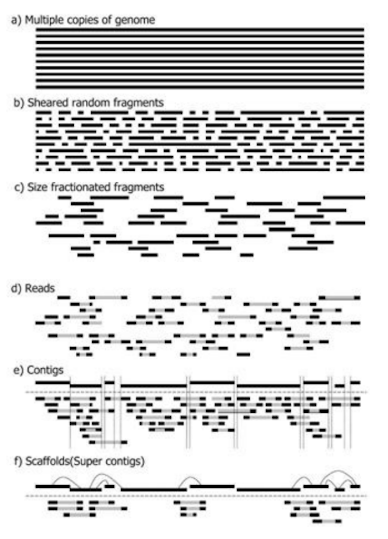
\includegraphics{images/genome_assembly.png}
\caption{Genome assembly}
\end{figure}

    Many genomes contain large numbers of repeat sequences. Often these
repeats are thousands of nucleotides long, and some occur in many
different locations in the genome. This makes genome assembly a very
difficult computational problem to solve. However, there are many genome
assembly tools that exist that can produce long contiguous sequences
(contigs) from sequencing reads. The assembly tool that you use will be
determined by different factors, largely this will be the length of the
sequencing reads and the sequencing technology used to produce the
reads.

In this practical we will assemble one chromosome of a malaria parasite:
Plasmodium falciparum, the IT clone. We have sequenced the genome with
both PacBio and Illumina and pre-filtered the reads to select only those
reads from a single chromosome.

\hypertarget{learning-outcomes}{%
\subsection{Learning outcomes}\label{learning-outcomes}}

On completion of the tutorial, you can expect to be able to:

\begin{itemize}
\tightlist
\item
  Describe the different approaches to genome assembly
\item
  Generate a genome assembly from illumina data
\item
  Generate a genome assembly from PacBio data
\item
  Generate statistics to evaluate the quality of a genome assembly
\item
  Estimate the size of a genome assembly
\end{itemize}

\hypertarget{tutorial-sections}{%
\subsection{Tutorial sections}\label{tutorial-sections}}

This tutorial comprises the following sections:\\
1. \href{pacbio_assembly.ipynb}{PacBio genome assembly}\\
2. \href{assembly_algorithms.ipynb}{Assembly algorithms}\\
3. \href{illumina_assembly.ipynb}{Illumina genome assembly} 4.
\href{assembly_estimation.ipynb}{Genome assembly estimation}\\
5. \href{pacbio_assembly_again.ipynb}{PacBio genome assembly again}

\hypertarget{authors}{%
\subsection{Authors}\label{authors}}

This tutorial was written by
\href{https://github.com/jacquikeane}{Jacqui Keane} based on material
from \href{https://github.com/mcshane}{Shane McCarthy} and Thomas Otto.

\hypertarget{running-the-commands-from-this-tutorial}{%
\subsection{Running the commands from this
tutorial}\label{running-the-commands-from-this-tutorial}}

You can follow this tutorial by typing all the commands you see into a
terminal window. This is similar to the ``Command Prompt'' window on MS
Windows systems, which allows the user to type DOS commands to manage
files.

To get started, open a new terminal window and type the command below:

    \begin{tcolorbox}[breakable, size=fbox, boxrule=1pt, pad at break*=1mm,colback=cellbackground, colframe=cellborder]
\prompt{In}{incolor}{1}{\boxspacing}
\begin{Verbatim}[commandchars=\\\{\}]
\PY{n+nb}{cd} \PYZti{}/course\PYZus{}data/assembly/data
\end{Verbatim}
\end{tcolorbox}

    \hypertarget{lets-get-started}{%
\subsection{Let's get started!}\label{lets-get-started}}

This tutorial requires that you have canu, jellyfish, velvet,
assembly-stats and wtdbg installed on your computer. These are already
installed on the virtual machine you are using. To check that these are
installed, run the following commands:

    \begin{tcolorbox}[breakable, size=fbox, boxrule=1pt, pad at break*=1mm,colback=cellbackground, colframe=cellborder]
\prompt{In}{incolor}{ }{\boxspacing}
\begin{Verbatim}[commandchars=\\\{\}]
canu
\end{Verbatim}
\end{tcolorbox}

    \begin{tcolorbox}[breakable, size=fbox, boxrule=1pt, pad at break*=1mm,colback=cellbackground, colframe=cellborder]
\prompt{In}{incolor}{ }{\boxspacing}
\begin{Verbatim}[commandchars=\\\{\}]
jellyfish
\end{Verbatim}
\end{tcolorbox}

    \begin{tcolorbox}[breakable, size=fbox, boxrule=1pt, pad at break*=1mm,colback=cellbackground, colframe=cellborder]
\prompt{In}{incolor}{ }{\boxspacing}
\begin{Verbatim}[commandchars=\\\{\}]
velvetg
\end{Verbatim}
\end{tcolorbox}

    \begin{tcolorbox}[breakable, size=fbox, boxrule=1pt, pad at break*=1mm,colback=cellbackground, colframe=cellborder]
\prompt{In}{incolor}{ }{\boxspacing}
\begin{Verbatim}[commandchars=\\\{\}]
velveth
\end{Verbatim}
\end{tcolorbox}

    \begin{tcolorbox}[breakable, size=fbox, boxrule=1pt, pad at break*=1mm,colback=cellbackground, colframe=cellborder]
\prompt{In}{incolor}{ }{\boxspacing}
\begin{Verbatim}[commandchars=\\\{\}]
assembly\PYZhy{}stats
\end{Verbatim}
\end{tcolorbox}

    \begin{tcolorbox}[breakable, size=fbox, boxrule=1pt, pad at break*=1mm,colback=cellbackground, colframe=cellborder]
\prompt{In}{incolor}{ }{\boxspacing}
\begin{Verbatim}[commandchars=\\\{\}]
wtdbg2
\end{Verbatim}
\end{tcolorbox}

    This should return the help message for software canu, jellyfish,
velvet, assembly-stats and wtdbg2 respectively.

If after this course you would like to download and install this
software the instructions can be found at the links below, alternatively
we recommend \href{https://bioconda.github.io/}{bioconda} for the
installation and management of your bioinformatics software.

\begin{itemize}
\tightlist
\item
  The \href{https://canu.readthedocs.io/en/latest/}{canu} website
\item
  The \href{https://github.com/gmarcais/Jellyfish}{jellyfish} github
  page
\item
  The \href{https://www.ebi.ac.uk/~zerbino/velvet/}{velvet} wesite
\item
  The \href{https://github.com/ruanjue/wtdbg2}{wtdbg2} github page
\end{itemize}

To get started with the tutorial, go to the first section:
\href{pacbio_assembly.ipynb}{Pacbio genome assembly}


    % Add a bibliography block to the postdoc



\newpage





    \hypertarget{pacbio-genome-assembly}{%
\section{PacBio Genome Assembly}\label{pacbio-genome-assembly}}

First, check you are in the correct directory.

    \begin{tcolorbox}[breakable, size=fbox, boxrule=1pt, pad at break*=1mm,colback=cellbackground, colframe=cellborder]
\prompt{In}{incolor}{ }{\boxspacing}
\begin{Verbatim}[commandchars=\\\{\}]
\PY{n+nb}{pwd}
\end{Verbatim}
\end{tcolorbox}

    It should display something like:

\texttt{/home/manager/course\_data/assembly/data}

    Now we are going to start the PacBio assembly using the \texttt{canu}
program. It first corrects the reads and then uses the \texttt{Celera}
assembler to merge the long reads into contigs. To see the contents of
the directory, type:

    \begin{tcolorbox}[breakable, size=fbox, boxrule=1pt, pad at break*=1mm,colback=cellbackground, colframe=cellborder]
\prompt{In}{incolor}{ }{\boxspacing}
\begin{Verbatim}[commandchars=\\\{\}]
ls
\end{Verbatim}
\end{tcolorbox}

    The pre-filtered PacBio reads are called \texttt{PBReads.fastq.gz} -
take a look at the contents of this file.

    \begin{tcolorbox}[breakable, size=fbox, boxrule=1pt, pad at break*=1mm,colback=cellbackground, colframe=cellborder]
\prompt{In}{incolor}{ }{\boxspacing}
\begin{Verbatim}[commandchars=\\\{\}]
zless \PYZhy{}S PBReads.fastq.gz
\end{Verbatim}
\end{tcolorbox}

    What do you notice compared to the Illumina fastq files you have seen
previously?

Now we will start the assembly with \texttt{canu}
\href{https://canu.readthedocs.io/}{(https://canu.readthedocs.io/)}.

\textbf{NOTE:} This will take some time, so we will start it running now
in the background and hopefully it will complete while we work on the
other exercises.

    \begin{tcolorbox}[breakable, size=fbox, boxrule=1pt, pad at break*=1mm,colback=cellbackground, colframe=cellborder]
\prompt{In}{incolor}{ }{\boxspacing}
\begin{Verbatim}[commandchars=\\\{\}]
canu \PYZhy{}p PB \PYZhy{}d canu\PYZhy{}assembly \PYZhy{}s file.specs \PYZhy{}pacbio\PYZhy{}raw PBReads.fastq.gz \PY{p}{\PYZam{}}\PYZgt{} canu\PYZus{}log.txt \PY{p}{\PYZam{}}
\end{Verbatim}
\end{tcolorbox}

    The \texttt{-p} option sets the prefix of output files to PB, while the
\texttt{-d} option sets the output directory to \texttt{canu-assembly/}.
The \texttt{\&} at the end will set this command running in the
background while you work through the next sections of this practical.

Before we move on, let's just make sure the program is running. Use the
\texttt{top} or better \texttt{htop} command to show you all processes
running on your machine (type \texttt{q} to exit \texttt{top}). You
should hopefully see processes associated with \texttt{canu} running (or
maybe something called \texttt{meryl}). We can also check the
\texttt{canu\_log.txt} file where the \texttt{canu} logs will be
written. If we see error messages in the file, then something has gone
wrong.

    \begin{tcolorbox}[breakable, size=fbox, boxrule=1pt, pad at break*=1mm,colback=cellbackground, colframe=cellborder]
\prompt{In}{incolor}{ }{\boxspacing}
\begin{Verbatim}[commandchars=\\\{\}]
htop
\end{Verbatim}
\end{tcolorbox}

    \begin{tcolorbox}[breakable, size=fbox, boxrule=1pt, pad at break*=1mm,colback=cellbackground, colframe=cellborder]
\prompt{In}{incolor}{ }{\boxspacing}
\begin{Verbatim}[commandchars=\\\{\}]
less canu\PYZus{}log.txt
\end{Verbatim}
\end{tcolorbox}

    While the \texttt{canu} assembly is running, move on to the next
section: \href{assembly_algorithms.ipynb}{Assembly algorithms}


    % Add a bibliography block to the postdoc



\newpage





    \hypertarget{assembly-algorithms}{%
\section{Assembly algorithms}\label{assembly-algorithms}}

There are several approaches (algorithms) that can be used to generate a
set of contiguous sequences (contigs) from a set of DNA fragments
(reads). Two of the main approaches are:

\begin{itemize}
\item
  \textbf{Overlap Layout Consensus (OLC):} This approach looks at all
  pairs x,y of all reads and determines if there is a sufficient overlap
  of the two reads. If there is, then it bundles the stretches of
  overlap graphs into contigs. Examples of assembly software that use
  this approach are Falcon (PacBio), Canu(Pacbio, ONT), mnimap/miniasm.
\item
  \textbf{de Brujin graph (DBG):} This approach builds a graph of all
  subsequences of lenght k (k-mers). Examples of assembly software that
  use this approach are velvet, ABySS, SPAdes, wtdbg2.
\end{itemize}

    \begin{figure}
\centering
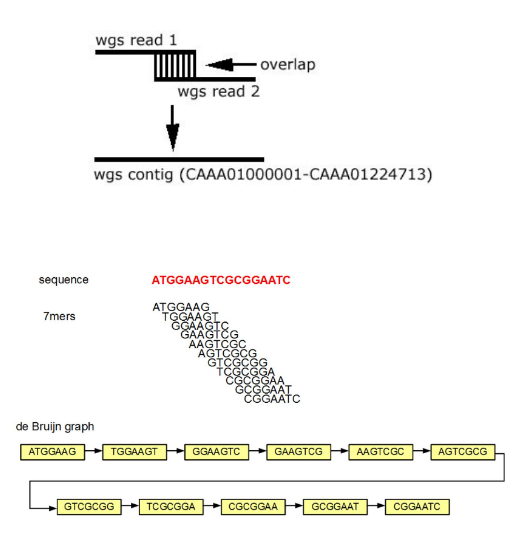
\includegraphics{images/assembly_algorithms.png}
\caption{Assembly algorithms}
\end{figure}

    \hypertarget{exercise}{%
\subsection{Exercise}\label{exercise}}

Here we are going to build a de Brujin graph by hand from a set of short
reads! Using the 6bp reads listed below, manually create the de Brujin
graph and find the contig(s).

    \begin{figure}
\centering
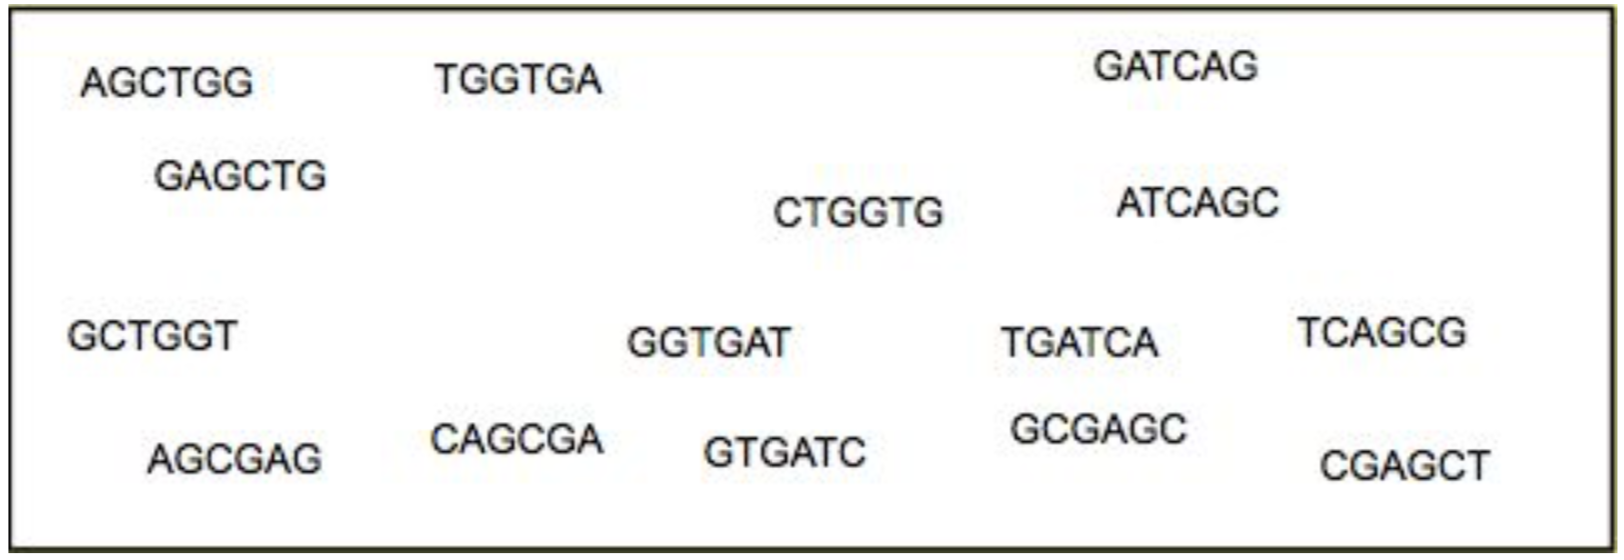
\includegraphics{images/debruijn1.png}
\caption{Short reads}
\end{figure}

    Using a k-mer value of k=5 produces the following k-mers of length 5
from the reads above. To finish the graph, join k-mers that overlap by 4
bases.

    \begin{figure}
\centering
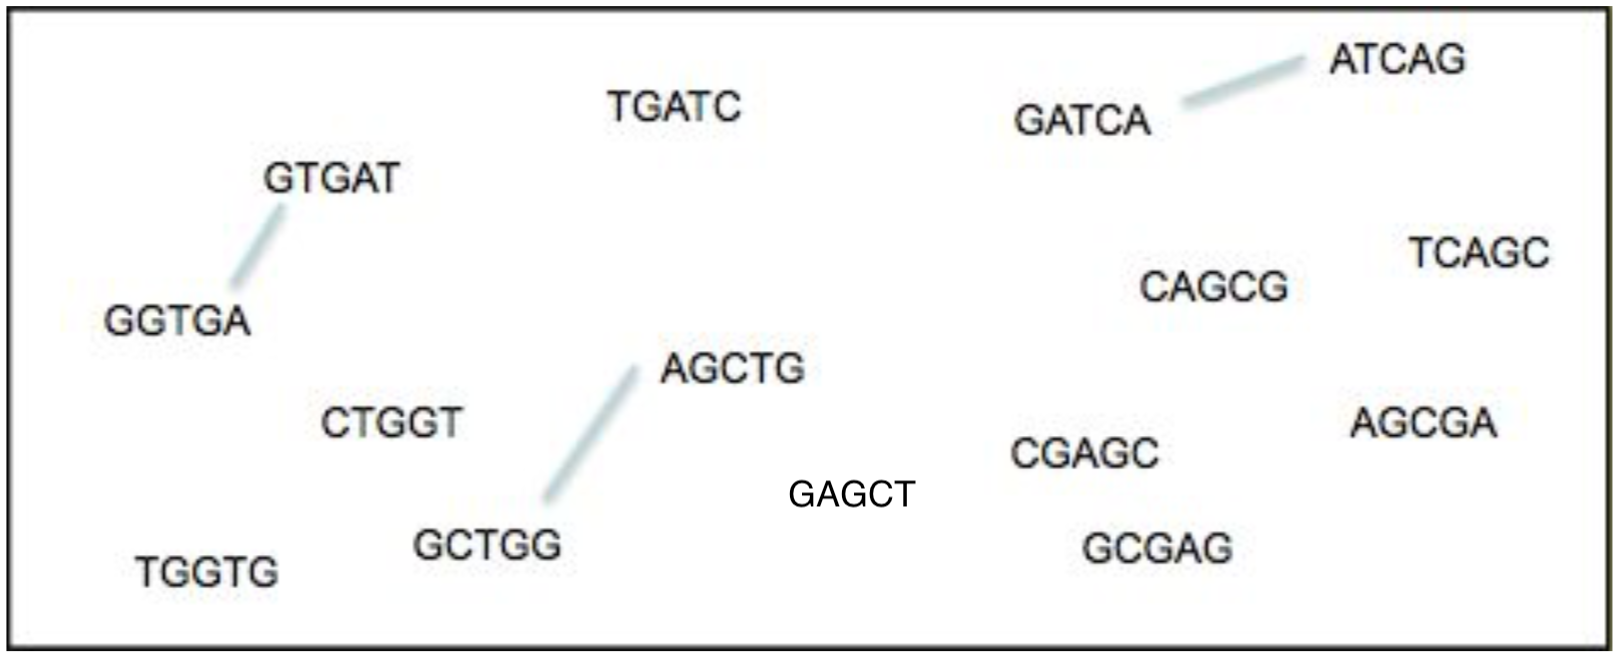
\includegraphics{images/debruijn2.png}
\caption{K-mers}
\end{figure}

    \textbf{Questions}

\begin{enumerate}
\def\labelenumi{\arabic{enumi}.}
\item
  What is the contig sequence?
\item
  What was difficult here?
\end{enumerate}

    Now move on to the next section: \href{illumina_assembly.ipynb}{Illumina
genome assembly}


    % Add a bibliography block to the postdoc



\newpage





    \hypertarget{illumina-genome-assembly}{%
\section{Illumina Genome Assembly}\label{illumina-genome-assembly}}

We are now going to use the assembler velvet
\url{https://www.ebi.ac.uk/~zerbino/velvet/} to assemble the Illumina
reads. Our Illumina reads are from the same sample we used to generate
the PacBio data.

    \hypertarget{generating-an-illumina-assembly-with-velvet}{%
\subsection{Generating an Illumina assembly with
velvet}\label{generating-an-illumina-assembly-with-velvet}}

Creating a genome assembly using velvet is a two stage process:

\begin{itemize}
\tightlist
\item
  First, the command \texttt{velveth} is used to generate the k-mers
  from the input data
\item
  Second, the command \texttt{velvetg} is used to build the de Bruijn
  graph and find the optimal path through the graph
\end{itemize}

To assemble the data, start with the command:

    \begin{tcolorbox}[breakable, size=fbox, boxrule=1pt, pad at break*=1mm,colback=cellbackground, colframe=cellborder]
\prompt{In}{incolor}{ }{\boxspacing}
\begin{Verbatim}[commandchars=\\\{\}]
velveth k.assembly.49 \PY{l+m}{49} \PYZhy{}shortPaired \PYZhy{}fastq IT.Chr5\PYZus{}1.fastq IT.Chr5\PYZus{}2.fastq
\end{Verbatim}
\end{tcolorbox}

    The input option \texttt{k.assembly.49} is the name of the directory
where the results are to be written. The vallue \texttt{49} is the k-mer
size. The other options specify the type of the input data
(\texttt{-shortPaired}) and \texttt{-fastq} is used to specify the fastq
files that contain the sequencing reads.

To see all possible options for velveth use:

    \begin{tcolorbox}[breakable, size=fbox, boxrule=1pt, pad at break*=1mm,colback=cellbackground, colframe=cellborder]
\prompt{In}{incolor}{ }{\boxspacing}
\begin{Verbatim}[commandchars=\\\{\}]
velveth
\end{Verbatim}
\end{tcolorbox}

    Now use velvetg to build the graph and find the path through the graph
(similar to what we did manually in the previous section):

    \begin{tcolorbox}[breakable, size=fbox, boxrule=1pt, pad at break*=1mm,colback=cellbackground, colframe=cellborder]
\prompt{In}{incolor}{ }{\boxspacing}
\begin{Verbatim}[commandchars=\\\{\}]
velvetg k.assembly.49 \PYZhy{}exp\PYZus{}cov auto \PYZhy{}ins\PYZus{}length \PY{l+m}{350}
\end{Verbatim}
\end{tcolorbox}

    The first parameter \texttt{k.assembly.49} specifies the working
directory as created with the \texttt{velveth} command. The second
\texttt{-exp\_cov\ auto} instructs velvet to find the median read
coverage automatically rather than specifying it yourself. Finally,
\texttt{-ins\_length} specifies the insert size of the sequencing
library used. There is a lot of output printed to the screen, but the
most important information is the last line:

\texttt{Final\ graph\ has\ 1455\ nodes\ and\ n50\ of\ 7527,\ max\ 38045,\ total\ 1364551,\ using\ 700301/770774\ reads.\ (Your\ exact\ result\ might\ differ\ depending\ on\ the\ velvet\ version\ used\ -\ don’t\ worry).}

This gives you a quick idea of the result.

\begin{itemize}
\tightlist
\item
  1455 nodes are in the final graph.
\item
  An n50 of 7527 means that 50\% of the assembly is in contigs of at
  least 7527 bases, it is the median contig size. This number is most
  commonly used as an indicator of assembly quality. The higher, the
  better! (but not always!)
\item
  Max is the length of the longest contig.
\item
  Total is the size of the assembly, here 1346kb.
\item
  The last two numbers tell us how many reads were used from the 7.7
  million pairs input data.
\end{itemize}

    To see all possible options for velvetg use:

    \begin{tcolorbox}[breakable, size=fbox, boxrule=1pt, pad at break*=1mm,colback=cellbackground, colframe=cellborder]
\prompt{In}{incolor}{ }{\boxspacing}
\begin{Verbatim}[commandchars=\\\{\}]
velvetg
\end{Verbatim}
\end{tcolorbox}

    Now let's try to improve the quality of the assembly by varying some of
the input parameters to velvet. Two parameters that can play a role in
improving the assembly are \texttt{-cov\_cutoff} and
\texttt{-min\_contig\_lgth}.

Using the \texttt{-cov\_cutoff} parameter means that nodes with less
than a specific k-mer count are removed from the graph.

Using the \texttt{-min\_contig\_lgth} parameter means that contigs with
less than a specific size are removed from the assembly.

Try re-running the assembly with a kmer of 49 and using a
\texttt{-cov\_cutoff} of 5 and \texttt{-min\_contig\_lgth} of 200.

    \begin{tcolorbox}[breakable, size=fbox, boxrule=1pt, pad at break*=1mm,colback=cellbackground, colframe=cellborder]
\prompt{In}{incolor}{ }{\boxspacing}
\begin{Verbatim}[commandchars=\\\{\}]
velvetg k.assembly.49 \PYZhy{}exp\PYZus{}cov auto \PYZhy{}ins\PYZus{}length \PY{l+m}{350} \PYZhy{}min\PYZus{}contig\PYZus{}lgth \PY{l+m}{200} \PYZhy{}cov\PYZus{}cutoff \PY{l+m}{5}
\end{Verbatim}
\end{tcolorbox}

    Note as we are not changing the k-mer size, we do not need run the
\texttt{velveth} command again.

    Generally, the k-mer size has the biggest impact on assembly results.
Let us make a few other assemblies for different k-mer sizes i.e.~55,
41. Here is the example for k-mer length of 55.

    \begin{tcolorbox}[breakable, size=fbox, boxrule=1pt, pad at break*=1mm,colback=cellbackground, colframe=cellborder]
\prompt{In}{incolor}{ }{\boxspacing}
\begin{Verbatim}[commandchars=\\\{\}]
velveth k.assembly.55 \PY{l+m}{55} \PYZhy{}shortPaired \PYZhy{}fastq IT.Chr5\PYZus{}1.fastq IT.Chr5\PYZus{}2.fastq
\end{Verbatim}
\end{tcolorbox}

    \begin{tcolorbox}[breakable, size=fbox, boxrule=1pt, pad at break*=1mm,colback=cellbackground, colframe=cellborder]
\prompt{In}{incolor}{ }{\boxspacing}
\begin{Verbatim}[commandchars=\\\{\}]
velvetg k.assembly.55 \PYZhy{}exp\PYZus{}cov auto \PYZhy{}ins\PYZus{}length \PY{l+m}{350} \PYZhy{}min\PYZus{}contig\PYZus{}lgth \PY{l+m}{200} \PYZhy{}cov\PYZus{}cutoff \PY{l+m}{5}
\end{Verbatim}
\end{tcolorbox}

    \textbf{Note:} If you find that you are having trouble running the
velvet assemblies or if it is running for longer than 10-15 mins then
quit the command (Ctrc-C). A pre-generated set of Illumina assemblies
can be found at:

    \begin{tcolorbox}[breakable, size=fbox, boxrule=1pt, pad at break*=1mm,colback=cellbackground, colframe=cellborder]
\prompt{In}{incolor}{ }{\boxspacing}
\begin{Verbatim}[commandchars=\\\{\}]
ls \PYZti{}/course\PYZus{}data/assembly/data/backup/illumina\PYZus{}assemblies
\end{Verbatim}
\end{tcolorbox}

    \hypertarget{assembly-metrics}{%
\subsection{Assembly metrics}\label{assembly-metrics}}

All the assembly results are written into the directory you specified
with the \texttt{velvet} commands,
e.g.~\texttt{k.assembly.41},\texttt{k.assembly.49},\texttt{k.assembly.55}.
The final contigs are written to a file called \texttt{contigs.fa}. The
\texttt{stats.txt} file holds some information about each contig, its
length, the coverage, etc. The other files contain information for the
assembler.

Another way to get more assembly statistics is to use a program called
\texttt{assembly-stats}. It displays the number of contigs, the mean
size and a lot of other useful statistics about the assembly. These
numbers can be used to assess the quality of your assemblies and help
you pick the ``best'' one.

Type:

    \begin{tcolorbox}[breakable, size=fbox, boxrule=1pt, pad at break*=1mm,colback=cellbackground, colframe=cellborder]
\prompt{In}{incolor}{ }{\boxspacing}
\begin{Verbatim}[commandchars=\\\{\}]
assembly\PYZhy{}stats k.assembly*/*.fa
\end{Verbatim}
\end{tcolorbox}

    \begin{figure}
\centering
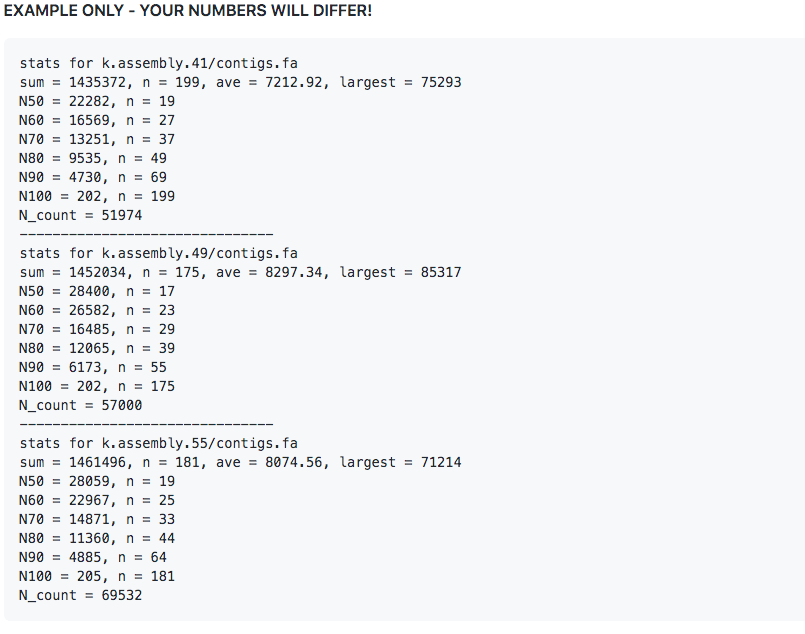
\includegraphics{images/assembly_stats_output.png}
\caption{Output from assembly stats}
\end{figure}

    Write down the results for each assembly made using different k-mer
sizes. Which one looks the best?

    \begin{figure}
\centering
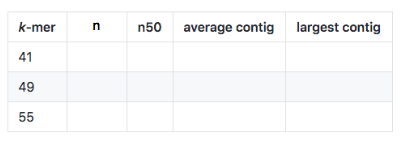
\includegraphics{images/velvet_stats.png}
\caption{Velvet assembly stats}
\end{figure}

    \textbf{Question:} What is the best choice for k?

We want to choose the set of parameters that produce the assembly where
the n50, average contig size and the largest contigs have the highest
values, while contig number is the lowest.

    You will notice another statistic produced by assembly-stats is
N\_count, what does the N\_count mean?

As we know, DNA templates can be sequenced from both ends, resulting in
mate pairs. Their outer distance is the insert size. Imagine mapping the
reads back onto the assembled contigs. In some cases the two mates don't
map onto the same contig. We can use those mates to scaffold the two
contigs e.g.~orientate them to each other and put N's between them, so
that the insert size is correct, if enough mate pairs suggest that join.
Velvet does this automatically (although you can turn it off). The
number of mates you need to join two contigs is defined by the parameter
\texttt{-min\_pair\_count}.

Here is the description:

    \texttt{-min\_pair\_count\ \textless{}integer\textgreater{}:\ minimum\ number\ of\ paired\ end\ connections\ to\ justify\ the\ scaffolding\ of\ two\ long\ contigs\ (default:\ 5)}

    Here is a schema:

    \begin{figure}
\centering
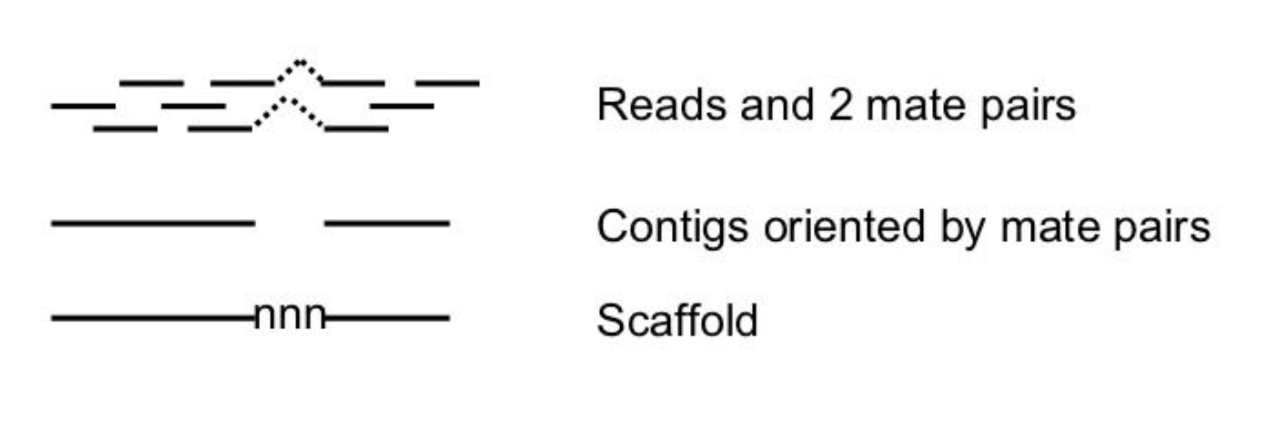
\includegraphics{images/schema.png}
\caption{Assembly scaffolds}
\end{figure}

    It might be worth mentioning, that incorrect scaffolding is the most
common source of error in assembly (so called mis-assemblies). If you
lower the min\_pair\_count too much, the likelihood of generating errors
increases.

Other errors are due to repeats. In a normal assembly one would expect
that the repeats are all collapsed, if they are smaller than the read
length. If the repeat unit is smaller than the insert size, than it is
possible to scaffold over it, leaving the space for the repeats with
N's.

To get the statistic for the contigs, rather than scaffolds
(supercontigs), you can use \texttt{seqtk} to break the scaffold at any
stretch of N's with the following commands:

    \begin{tcolorbox}[breakable, size=fbox, boxrule=1pt, pad at break*=1mm,colback=cellbackground, colframe=cellborder]
\prompt{In}{incolor}{ }{\boxspacing}
\begin{Verbatim}[commandchars=\\\{\}]
seqtk cutN \PYZhy{}n1 k.assembly.41/contigs.fa \PYZgt{} assembly.41.contigs.fasta
\end{Verbatim}
\end{tcolorbox}

    \begin{tcolorbox}[breakable, size=fbox, boxrule=1pt, pad at break*=1mm,colback=cellbackground, colframe=cellborder]
\prompt{In}{incolor}{ }{\boxspacing}
\begin{Verbatim}[commandchars=\\\{\}]
assembly\PYZhy{}stats assembly.41.contigs.fasta
\end{Verbatim}
\end{tcolorbox}

    \begin{tcolorbox}[breakable, size=fbox, boxrule=1pt, pad at break*=1mm,colback=cellbackground, colframe=cellborder]
\prompt{In}{incolor}{ }{\boxspacing}
\begin{Verbatim}[commandchars=\\\{\}]
seqtk cutN \PYZhy{}n1 k.assembly.49/contigs.fa \PYZgt{} assembly.49.contigs.fasta
\end{Verbatim}
\end{tcolorbox}

    \begin{tcolorbox}[breakable, size=fbox, boxrule=1pt, pad at break*=1mm,colback=cellbackground, colframe=cellborder]
\prompt{In}{incolor}{ }{\boxspacing}
\begin{Verbatim}[commandchars=\\\{\}]
assembly\PYZhy{}stats assembly.49.contigs.fasta
\end{Verbatim}
\end{tcolorbox}

    \begin{tcolorbox}[breakable, size=fbox, boxrule=1pt, pad at break*=1mm,colback=cellbackground, colframe=cellborder]
\prompt{In}{incolor}{ }{\boxspacing}
\begin{Verbatim}[commandchars=\\\{\}]
seqtk cutN \PYZhy{}n1 k.assembly.55/contigs.fa \PYZgt{} assembly.55.contigs.fasta
\end{Verbatim}
\end{tcolorbox}

    \begin{tcolorbox}[breakable, size=fbox, boxrule=1pt, pad at break*=1mm,colback=cellbackground, colframe=cellborder]
\prompt{In}{incolor}{ }{\boxspacing}
\begin{Verbatim}[commandchars=\\\{\}]
assembly\PYZhy{}stats assembly.55.contigs.fasta
\end{Verbatim}
\end{tcolorbox}

    \textbf{Question:} How does the contig N50 compare to the scaffold N50
for each of your assemblies?

    \begin{figure}
\centering
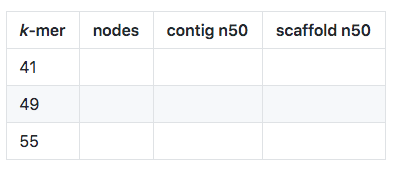
\includegraphics{images/n50_comparisons.png}
\caption{Output from assembly stats for velvet contigs}
\end{figure}

    Congratulations you have sucessfully created a genome assembly using
Illumina sequence data. Now move on to the next section:
\href{assembly_estimation.ipynb}{Assembly estimation}


    % Add a bibliography block to the postdoc



\newpage





    \hypertarget{assembly-estimation}{%
\section{Assembly estimation}\label{assembly-estimation}}

Fortunately with this dataset, we have a known reference genome and
therefore some expectations about the size and composition of the
Plasmodium falciparum genome.

But what if we are working with a new genome, one which has not been
sequenced before? One approach is to look at k-mer distributions from
the reads. This can be done using two pieces of software,
\texttt{jellyfish}
\href{https://github.com/gmarcais/Jellyfish}{(https://github.com/gmarcais/Jellyfish)}
and \texttt{Genomesope}
\href{http://qb.cshl.edu/genomescope/}{(http://qb.cshl.edu/genomescope/)}.
\texttt{Jellyfish} is used to determine the distribution of k-mers in
the dataset and then \texttt{Genomescope} is used to model the single
copy k-mers as heterozygotes, while double copy k-mers will be the
homozygous portions of the genome. It will also estimate the haploid
genome size.

Let's check with our Plasmodium falciparum Illumina data that the k-mer
distribution gives us what we expect. To get a distribution of 21-mers:

    \begin{tcolorbox}[breakable, size=fbox, boxrule=1pt, pad at break*=1mm,colback=cellbackground, colframe=cellborder]
\prompt{In}{incolor}{ }{\boxspacing}
\begin{Verbatim}[commandchars=\\\{\}]
jellyfish count \PYZhy{}C \PYZhy{}m \PY{l+m}{21} \PYZhy{}s 1G \PYZhy{}t \PY{l+m}{2} \PYZhy{}o IT.jf \PYZlt{}\PY{o}{(}cat IT.Chr5\PYZus{}1.fastq IT.Chr5\PYZus{}2.fastq\PY{o}{)}
\end{Verbatim}
\end{tcolorbox}

    This command will count canonical (\texttt{-C}) 21-mers
(\texttt{-m\ 21}), using a hash with 1G elements (\texttt{-s\ 1G}) and 2
threads (\texttt{-t\ 2}). The output is written to \texttt{IT.jf}.

    To compute the histogram of the k-mer occurences, use

    \begin{tcolorbox}[breakable, size=fbox, boxrule=1pt, pad at break*=1mm,colback=cellbackground, colframe=cellborder]
\prompt{In}{incolor}{ }{\boxspacing}
\begin{Verbatim}[commandchars=\\\{\}]
jellyfish histo IT.jf \PYZgt{} IT.histo
\end{Verbatim}
\end{tcolorbox}

    Look at the output:

    \begin{tcolorbox}[breakable, size=fbox, boxrule=1pt, pad at break*=1mm,colback=cellbackground, colframe=cellborder]
\prompt{In}{incolor}{ }{\boxspacing}
\begin{Verbatim}[commandchars=\\\{\}]
less IT.histo
\end{Verbatim}
\end{tcolorbox}

    Now analyse the output with \texttt{genomescope}:

    \begin{tcolorbox}[breakable, size=fbox, boxrule=1pt, pad at break*=1mm,colback=cellbackground, colframe=cellborder]
\prompt{In}{incolor}{ }{\boxspacing}
\begin{Verbatim}[commandchars=\\\{\}]
Rscript genomescope.R IT.histo \PY{l+m}{21} \PY{l+m}{76} IT.jf21
\end{Verbatim}
\end{tcolorbox}

    Where 21 is the k-mer size, 76 is the read length of the input Illumina
data and IT.jf21 is the directory to write the output to. To look at the
output use:

    \begin{tcolorbox}[breakable, size=fbox, boxrule=1pt, pad at break*=1mm,colback=cellbackground, colframe=cellborder]
\prompt{In}{incolor}{ }{\boxspacing}
\begin{Verbatim}[commandchars=\\\{\}]
less IT.jf21/summary.txt
\end{Verbatim}
\end{tcolorbox}

    \begin{tcolorbox}[breakable, size=fbox, boxrule=1pt, pad at break*=1mm,colback=cellbackground, colframe=cellborder]
\prompt{In}{incolor}{ }{\boxspacing}
\begin{Verbatim}[commandchars=\\\{\}]
firefox IT.jf21/plot.png \PY{p}{\PYZam{}}
\end{Verbatim}
\end{tcolorbox}

    You should see an image similar to the ones shown below. Notice the bump
to right of the main peak. These are the repeated sequences.

    \hypertarget{exercises}{%
\subsection{Exercises}\label{exercises}}

\begin{enumerate}
\def\labelenumi{\arabic{enumi}.}
\tightlist
\item
  What is the predicted heterozygosity?
\item
  What is the predicted genome size?
\item
  Does this seem reasonable?
\end{enumerate}

    We have used \texttt{jellyfish} to pre-generate a set of k-mer
histograms for a handful of other species. These histo files can be
found in the data directory.

    \begin{tcolorbox}[breakable, size=fbox, boxrule=1pt, pad at break*=1mm,colback=cellbackground, colframe=cellborder]
\prompt{In}{incolor}{ }{\boxspacing}
\begin{Verbatim}[commandchars=\\\{\}]
ls *.histo
\end{Verbatim}
\end{tcolorbox}

    Try running genomscope on these. The read length for all of the datasets
is 150bp.

\textbf{fAnaTes1.jf21.histo:} What is the bulge to the left of the main
peak here?

    \begin{tcolorbox}[breakable, size=fbox, boxrule=1pt, pad at break*=1mm,colback=cellbackground, colframe=cellborder]
\prompt{In}{incolor}{ }{\boxspacing}
\begin{Verbatim}[commandchars=\\\{\}]
Rscript genomescope.R fAnaTes1.jf21.histo \PY{l+m}{21} \PY{l+m}{150} fAnaTes1.jf21
\end{Verbatim}
\end{tcolorbox}

    \textbf{fDreSAT1.jf21.histo:} What is the striking feature of this
genome?

\textbf{fMasArm1.jf21.histo:} You should see a nice tight diploid peak
for this sample. It has very low heterozygosity - similar to human data.

\textbf{fSalTru1.jf21.histo:} This genome was actually haploid. How do
we interpret the features in the genomescope profile?

    \begin{figure}
\centering
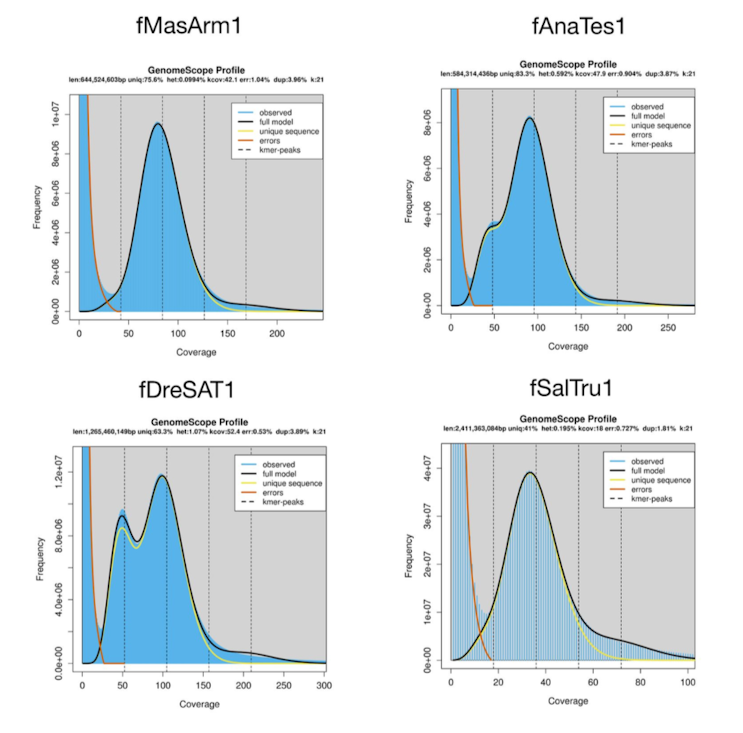
\includegraphics{images/gscope_examples.png}
\caption{Genomescope examples}
\end{figure}

    Now let us go back to our PacBio assembly:
\href{pacbio_assembly_again.ipynb}{PacBio assembly}


    % Add a bibliography block to the postdoc



\newpage





    \hypertarget{pacbio-genome-assembly-contd.}{%
\section{PacBio Genome Assembly
contd.}\label{pacbio-genome-assembly-contd.}}

We have generated an assembly for the Plasmodium falciparum chromosome
from our Illumina data. Now, let's have a look at the PacBio assembly.

\hypertarget{generating-pacbio-assemblies}{%
\subsection{Generating pacbio
assemblies}\label{generating-pacbio-assemblies}}

The \texttt{canu} pacbio assembly should have hopefully finished by now
(check the log less canu\_log.txt).

If it has not finished, you can find a pre-generated canu assembly at:

    \begin{tcolorbox}[breakable, size=fbox, boxrule=1pt, pad at break*=1mm,colback=cellbackground, colframe=cellborder]
\prompt{In}{incolor}{ }{\boxspacing}
\begin{Verbatim}[commandchars=\\\{\}]
ls \PYZti{}/course\PYZus{}data/assembly/data/backup/pacbio\PYZus{}assemblies
\end{Verbatim}
\end{tcolorbox}

    Now use the \texttt{assembly-stats} script to look at the assembly
statistics.

    \begin{tcolorbox}[breakable, size=fbox, boxrule=1pt, pad at break*=1mm,colback=cellbackground, colframe=cellborder]
\prompt{In}{incolor}{ }{\boxspacing}
\begin{Verbatim}[commandchars=\\\{\}]
assembly\PYZhy{}stats canu\PYZhy{}assembly/PB.contigs.fasta
\end{Verbatim}
\end{tcolorbox}

    How does it compare to the Illumina assembly?

    Another long read assembler based on de Bruijn graphs is \texttt{wtdbg2}
\url{https://github.com/ruanjue/wtdbg2}. Let's try to build a second
assembly using this assembler and compare it to the assembly produced
with \texttt{canu}.

    \begin{tcolorbox}[breakable, size=fbox, boxrule=1pt, pad at break*=1mm,colback=cellbackground, colframe=cellborder]
\prompt{In}{incolor}{ }{\boxspacing}
\begin{Verbatim}[commandchars=\\\{\}]
wtdbg2 \PYZhy{}t2 \PYZhy{}i PBReads.fastq.gz \PYZhy{}o wtdbg
\end{Verbatim}
\end{tcolorbox}

    \begin{tcolorbox}[breakable, size=fbox, boxrule=1pt, pad at break*=1mm,colback=cellbackground, colframe=cellborder]
\prompt{In}{incolor}{ }{\boxspacing}
\begin{Verbatim}[commandchars=\\\{\}]
wtpoa\PYZhy{}cns \PYZhy{}t2 \PYZhy{}i wtdbg.ctg.lay.gz \PYZhy{}fo wtdbg.ctg.lay.fasta
\end{Verbatim}
\end{tcolorbox}

    \begin{tcolorbox}[breakable, size=fbox, boxrule=1pt, pad at break*=1mm,colback=cellbackground, colframe=cellborder]
\prompt{In}{incolor}{ }{\boxspacing}
\begin{Verbatim}[commandchars=\\\{\}]
assembly\PYZhy{}stats wtdbg.ctg.lay.fasta
\end{Verbatim}
\end{tcolorbox}

    \hypertarget{comparing-pacbio-assemblies}{%
\subsection{Comparing pacbio
assemblies}\label{comparing-pacbio-assemblies}}

How does the wtdbg2 assembly compare to the canu assembly? Both
assemblies may be similar in contig number and N50, but are they really
similar? Let's map the Illumina reads to each assembly, call variants
and compare.

    \begin{tcolorbox}[breakable, size=fbox, boxrule=1pt, pad at break*=1mm,colback=cellbackground, colframe=cellborder]
\prompt{In}{incolor}{ }{\boxspacing}
\begin{Verbatim}[commandchars=\\\{\}]
bwa index canu\PYZhy{}assembly/PB.contigs.fasta
\end{Verbatim}
\end{tcolorbox}

    \begin{tcolorbox}[breakable, size=fbox, boxrule=1pt, pad at break*=1mm,colback=cellbackground, colframe=cellborder]
\prompt{In}{incolor}{ }{\boxspacing}
\begin{Verbatim}[commandchars=\\\{\}]
samtools faidx canu\PYZhy{}assembly/PB.contigs.fasta
\end{Verbatim}
\end{tcolorbox}

    \begin{tcolorbox}[breakable, size=fbox, boxrule=1pt, pad at break*=1mm,colback=cellbackground, colframe=cellborder]
\prompt{In}{incolor}{ }{\boxspacing}
\begin{Verbatim}[commandchars=\\\{\}]
bwa mem \PYZhy{}t2 canu\PYZhy{}assembly/PB.contigs.fasta IT.Chr5\PYZus{}1.fastq IT.Chr5\PYZus{}2.fastq \PY{p}{|} samtools sort \PYZhy{}@2 \PYZhy{} \PY{p}{|} samtools mpileup \PYZhy{}f canu\PYZhy{}assembly/PB.contigs.fasta \PYZhy{}ug \PYZhy{} \PY{p}{|} bcftools call \PYZhy{}mv \PYZgt{} canu.vcf
\end{Verbatim}
\end{tcolorbox}

    Do the same for \texttt{wtdbg.ctg.lay.fasta} and then compare some basic
statistics.

    \begin{tcolorbox}[breakable, size=fbox, boxrule=1pt, pad at break*=1mm,colback=cellbackground, colframe=cellborder]
\prompt{In}{incolor}{ }{\boxspacing}
\begin{Verbatim}[commandchars=\\\{\}]
bwa index wtdbg.ctg.lay.fasta
\end{Verbatim}
\end{tcolorbox}

    \begin{tcolorbox}[breakable, size=fbox, boxrule=1pt, pad at break*=1mm,colback=cellbackground, colframe=cellborder]
\prompt{In}{incolor}{ }{\boxspacing}
\begin{Verbatim}[commandchars=\\\{\}]
samtools faidx wtdbg.ctg.lay.fasta
\end{Verbatim}
\end{tcolorbox}

    \begin{tcolorbox}[breakable, size=fbox, boxrule=1pt, pad at break*=1mm,colback=cellbackground, colframe=cellborder]
\prompt{In}{incolor}{ }{\boxspacing}
\begin{Verbatim}[commandchars=\\\{\}]
bwa mem \PYZhy{}t2 wtdbg.ctg.lay.fasta IT.Chr5\PYZus{}1.fastq IT.Chr5\PYZus{}2.fastq \PY{p}{|} samtools sort \PYZhy{}@2 \PYZhy{} \PY{p}{|} samtools mpileup \PYZhy{}f wtdbg.ctg.lay.fasta \PYZhy{}ug \PYZhy{} \PY{p}{|} bcftools call \PYZhy{}mv \PYZgt{} wtdbg.vcf
\end{Verbatim}
\end{tcolorbox}

    \begin{tcolorbox}[breakable, size=fbox, boxrule=1pt, pad at break*=1mm,colback=cellbackground, colframe=cellborder]
\prompt{In}{incolor}{ }{\boxspacing}
\begin{Verbatim}[commandchars=\\\{\}]
bcftools stats canu.vcf \PY{p}{|} grep \PYZca{}SN
\end{Verbatim}
\end{tcolorbox}

    \begin{tcolorbox}[breakable, size=fbox, boxrule=1pt, pad at break*=1mm,colback=cellbackground, colframe=cellborder]
\prompt{In}{incolor}{ }{\boxspacing}
\begin{Verbatim}[commandchars=\\\{\}]
bcftools stats wtdbg.vcf \PY{p}{|} grep \PYZca{}SN
\end{Verbatim}
\end{tcolorbox}

    \textbf{Question:} What do you notice in terms of the number of SNP and
indel calls?

The \texttt{wtdbg2} assembly has more variants due to having more
errors. This is mainly due to a lack of polishing or error correction -
something that the \texttt{canu} assembler performs, but the
\texttt{wtdbg2} assembler does not.

    \hypertarget{polishing-pacbio-assembly}{%
\subsection{Polishing pacbio assembly}\label{polishing-pacbio-assembly}}

Correcting errors is an important step in making an assembly, especially
from noisy long ready data. Not polishing an assembly can lead to genes
not being identified due to insertion and deletion errors in the
assembly sequence. To polish a genome assembly with Illumina data we use
\texttt{bcftools\ consensus} to change homozygous differences between
the assembly and the Illumina data to match the Illumina data

    Run the following steps to polish the \texttt{canu} assembly

    \begin{tcolorbox}[breakable, size=fbox, boxrule=1pt, pad at break*=1mm,colback=cellbackground, colframe=cellborder]
\prompt{In}{incolor}{ }{\boxspacing}
\begin{Verbatim}[commandchars=\\\{\}]
bgzip \PYZhy{}c canu.vcf \PYZgt{} canu.vcf.gz
\end{Verbatim}
\end{tcolorbox}

    \begin{tcolorbox}[breakable, size=fbox, boxrule=1pt, pad at break*=1mm,colback=cellbackground, colframe=cellborder]
\prompt{In}{incolor}{ }{\boxspacing}
\begin{Verbatim}[commandchars=\\\{\}]
tabix canu.vcf.gz
\end{Verbatim}
\end{tcolorbox}

    \begin{tcolorbox}[breakable, size=fbox, boxrule=1pt, pad at break*=1mm,colback=cellbackground, colframe=cellborder]
\prompt{In}{incolor}{ }{\boxspacing}
\begin{Verbatim}[commandchars=\\\{\}]
bcftools consensus \PYZhy{}i\PY{l+s+s1}{\PYZsq{}QUAL\PYZgt{}1 \PYZam{}\PYZam{} (GT=\PYZdq{}AA\PYZdq{} || GT=\PYZdq{}Aa\PYZdq{})\PYZsq{}} \PYZhy{}Hla \PYZhy{}f canu\PYZhy{}assembly/PB.contigs.fasta canu.vcf.gz \PYZgt{} canu\PYZhy{}assembly/PB.contigs.polished.fasta
\end{Verbatim}
\end{tcolorbox}

    \begin{tcolorbox}[breakable, size=fbox, boxrule=1pt, pad at break*=1mm,colback=cellbackground, colframe=cellborder]
\prompt{In}{incolor}{ }{\boxspacing}
\begin{Verbatim}[commandchars=\\\{\}]
Run the following steps to polish the \PY{l+s+sb}{`}wtdbg2\PY{l+s+sb}{`} assembly
\end{Verbatim}
\end{tcolorbox}

    \begin{tcolorbox}[breakable, size=fbox, boxrule=1pt, pad at break*=1mm,colback=cellbackground, colframe=cellborder]
\prompt{In}{incolor}{ }{\boxspacing}
\begin{Verbatim}[commandchars=\\\{\}]
bgzip \PYZhy{}c wtdbg.vcf \PYZgt{} wtdbg.vcf.gz
\end{Verbatim}
\end{tcolorbox}

    \begin{tcolorbox}[breakable, size=fbox, boxrule=1pt, pad at break*=1mm,colback=cellbackground, colframe=cellborder]
\prompt{In}{incolor}{ }{\boxspacing}
\begin{Verbatim}[commandchars=\\\{\}]
tabix wtdbg.vcf.gz
\end{Verbatim}
\end{tcolorbox}

    \begin{tcolorbox}[breakable, size=fbox, boxrule=1pt, pad at break*=1mm,colback=cellbackground, colframe=cellborder]
\prompt{In}{incolor}{ }{\boxspacing}
\begin{Verbatim}[commandchars=\\\{\}]
bcftools consensus \PYZhy{}i\PY{l+s+s1}{\PYZsq{}QUAL\PYZgt{}1 \PYZam{}\PYZam{} (GT=\PYZdq{}AA\PYZdq{} || GT=\PYZdq{}Aa\PYZdq{})\PYZsq{}} \PYZhy{}Hla \PYZhy{}f wtdbg.ctg.lay.fasta wtdbg.vcf.gz \PYZgt{} wtdbg.contigs.polished.fasta
\end{Verbatim}
\end{tcolorbox}

    Finally, align and call variants like before (bwa index/bwa
mem/samtools-sort/mpileup/bcftools call) using the polished assemblies
as the reference this time.

When running this analysis on these polished genomes, do we still get
variants? More or less than with the raw \texttt{canu} and
\texttt{wtdbg2} assemblies? Why?

    Congratulations, you have reached the end of the Genome Assembly
tutorial.


    % Add a bibliography block to the postdoc



\end{document}
